\section{Circuit}
\subsection{Level detector}
Here the main board is an esp8266 not the arduino uno.\\
The circuit schematic is as follows:\\
%\includegraphics[width=\textwidth]{schematic}
\begin{center}
    \begin{tabular}{|c|c|}
        \hline
        Device             & pinout \\
        \hline
        \hline
        Sonar vcc & Vin     \\
        \hline
        Echo                & D1      \\
        \hline
        Trig                 & D0      \\
        \hline
        Green Anode                 & D2      \\
        \hline
        Red Anode                 & D3      \\
        \hline
        Red cathode              & 220ohm to ground      \\
        \hline
        Green cathode              & 220ohm to ground     \\
        \hline
    \end{tabular}
\end{center}
Since the sonar works at 5 volt its vcc pin has to be fed by the vin of the esp8266, it is directly liked to the 5v line of the usb, otherwise it would get only 3.3 that is the working tension of the microcontorller.
\pagebreak

\subsection{Water channel controller}
The circuit schematic is as follows:\\
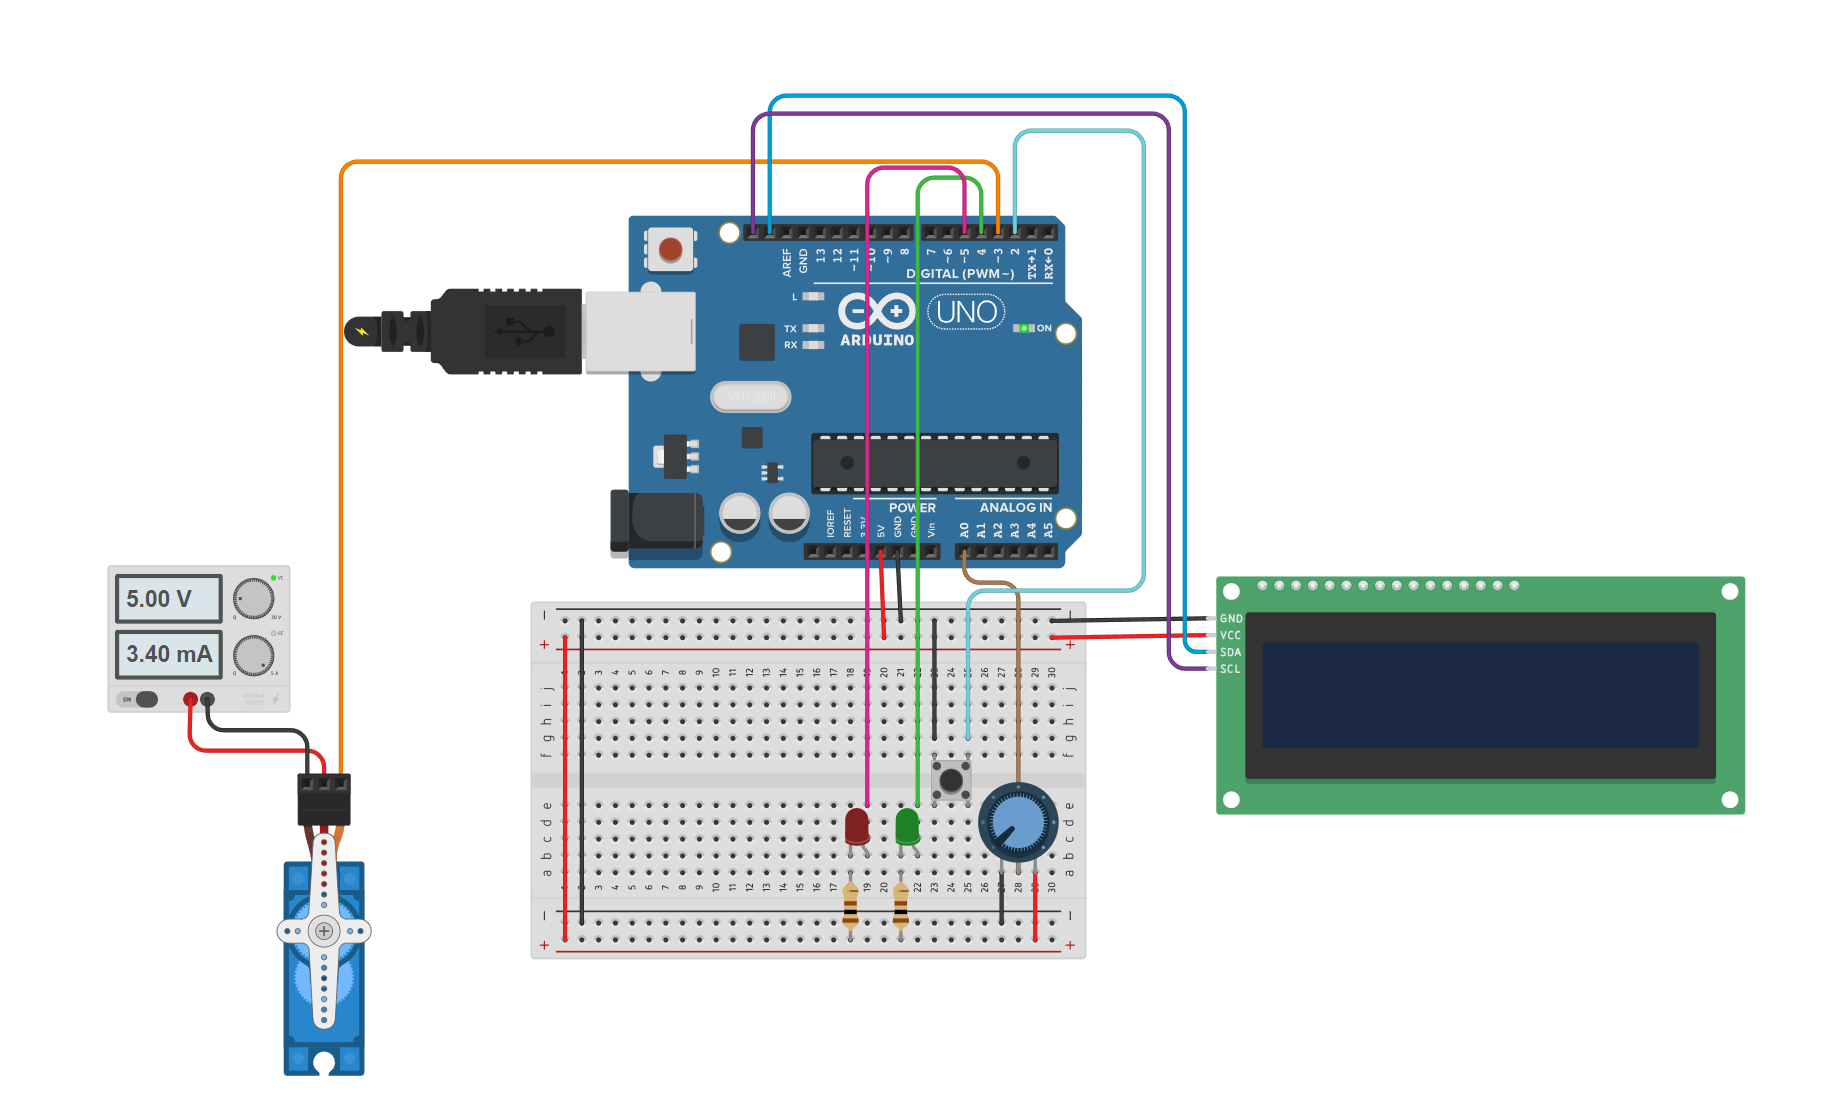
\includegraphics[width=\textwidth]{circuit.png}
\begin{center}
    \begin{tabular}{|c|c|}
        \hline
        Device             & pinout \\
        \hline
        \hline
        Servo vcc/gnd  & ext power supply     \\
        \hline
        Servo signal                &    3   \\
        \hline
        Button                 & 2      \\
        \hline
        Green Anode                 & 4      \\
        \hline
        Red Anode                 & 5      \\
        \hline
        Red cathode              & 220ohm to ground      \\
        \hline
        Green cathode              & 220ohm to ground     \\
        \hline
        Potentiometer              & A0     \\
        \hline
        LCD  SDA             & SDA     \\
        \hline
        LCD  SCL             & SCL     \\
        \hline
    \end{tabular}
\end{center}
The button is configured as input pullup, so it does not require an external resistor.
The servo is fed by an external power supply since it needs peaks of current that the arduino is not capable of offering without some additional capacitors. 
\pagebreak


\section{Software Architecture}
\subsection{Water Level Monitoring subsystem}
This segment of the system is composed by a simple arduino sketch that sends the readings of the sonar to a mqtt topic.\\
It also reads the required frequency of the recordings in another topic, this frequency is set by the main service (see below).
\subsection{Dashboard}
The dashboard is written in html css an js, it is packaged in a runnable executable exploiting the electron framework.\\
It fetches the data via http with a the get method, the main service sends the parameter in a json format.\\
It sets the parameter with a post request sending data in json format as well. \\
From the dashboard it is possible to select the mode and the position of the valve.\\
It also shows the actual level of the water and a chart of the past values.
\begin{figure}[H]
    \centering
    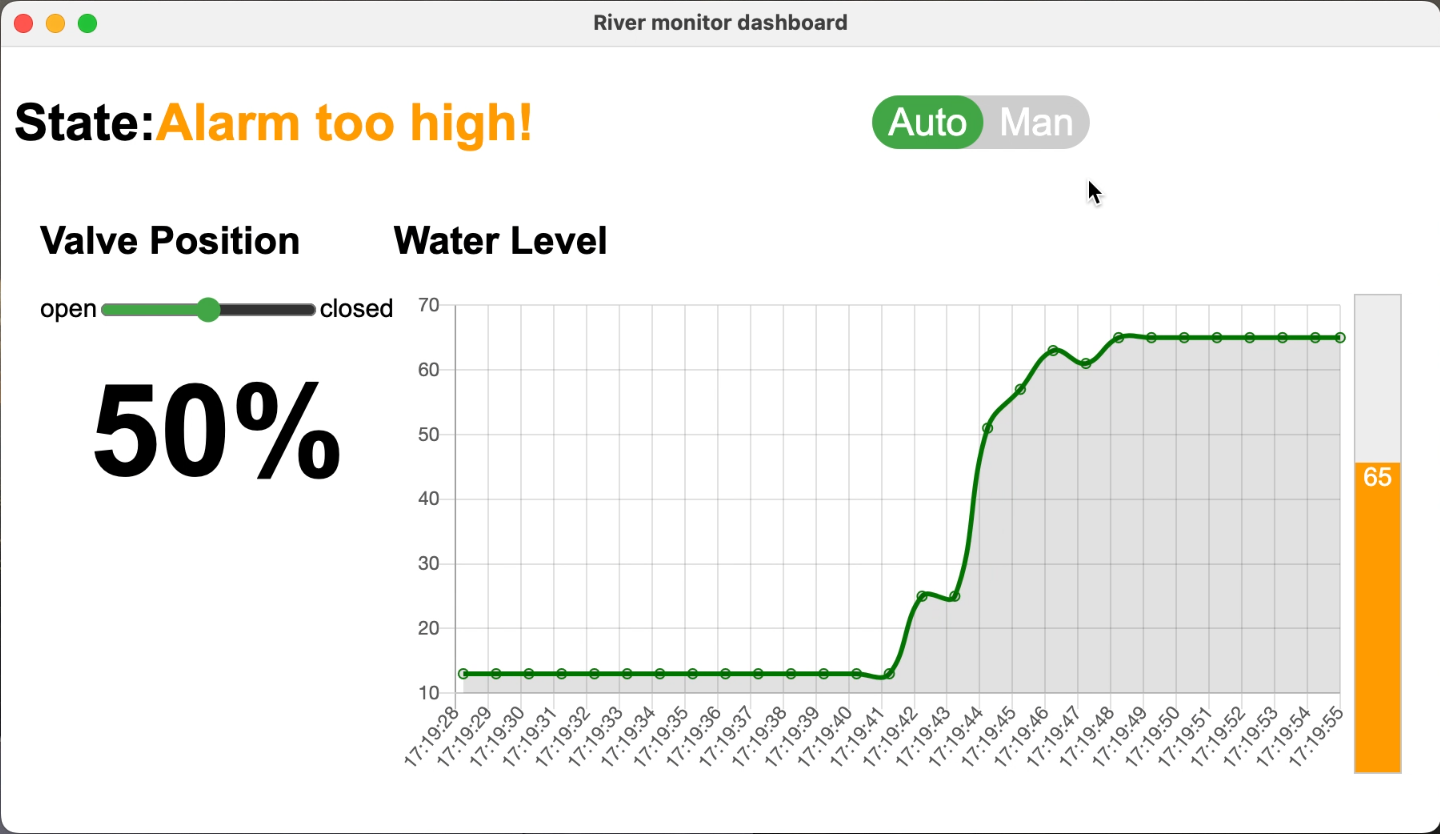
\includegraphics[width=\textwidth]{Screenshot.png}
\end{figure}
\pagebreak
\subsection{River Monitoring Service}
This is the main service that manages the logic of the system, it follows the specs given by the assignment.\\
It is written in js and run by node, it communicates with arduino exchanging data on the serial line. It fetches the level of the water via mqtt.\\
Via express.js it exposes the API with get and post methods to set and get the data.
\subsection{Water Channel Controller}
The program running on arduino is written in C++ using the wiring framework and the platformIo utility.\\
It is managed by a syncronous scheduler, it is triggered by a timer and launches non cooperative tasks.\\
Each task period has been chosen accordingly to its operative requirements, and is a multiple of the base period of the scheduler.
Some empiric tests have been made to ensure that no overrun happens in any scenario.\\
The work tree of the program is divided in:
\begin{itemize}
    \item Sensors, containing interfaces (abstract classes) and implementations for the devices.
    \item actuators, containing interfaces (abstract classes) and implementations for the devices.
    \item System, containing the scheduler and the task interface.
    \item Task, containing all the tasks.
\end{itemize}
On the root are present:
\begin{itemize}
    \item The main file, entry poit of the program, where the scheduler and the tasks are instantiated.
    \item Smart river monitoring class, representing the domain of the system with all the shared variables.
    \item Config, configuration file to tune all the parameters of the program.
\end{itemize}
\pagebreak

\section{Tasks}
\subsection{communicator Task}
This task is responsible of communicating via serial with the dashboard encoding in json the relative data.\\
It also collects the request incoming via serial in the same format.
\begin{figure}[H]
    \centering
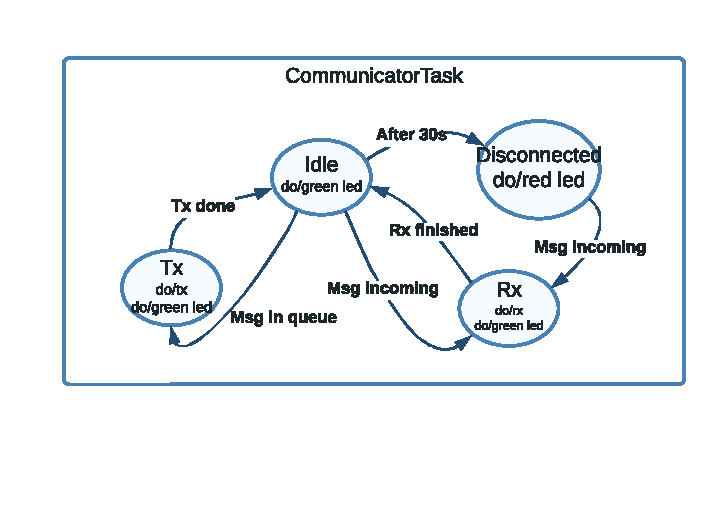
\includegraphics[width=0.9\textwidth]{Communicator.pdf}
\end{figure}
\pagebreak
\subsection{valveController Task}
This task is responsible of change the position of the valve according to the instructions fetched from the other tasks.
\begin{figure}[H]
    \centering
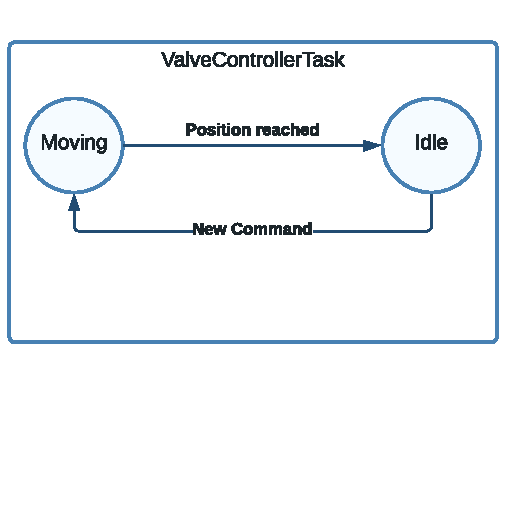
\includegraphics[width=0.6\textwidth]{ValveController.pdf}
\end{figure}
\subsection{inputChecker Task}
This task is responsible of sensing the changes in the potentiometer and on the button, it issues commands accordingly.
It automatically switches to manual if the potentiometer is moved, while for the button it alternates between the two modes.
\begin{figure}[H]
    \centering
%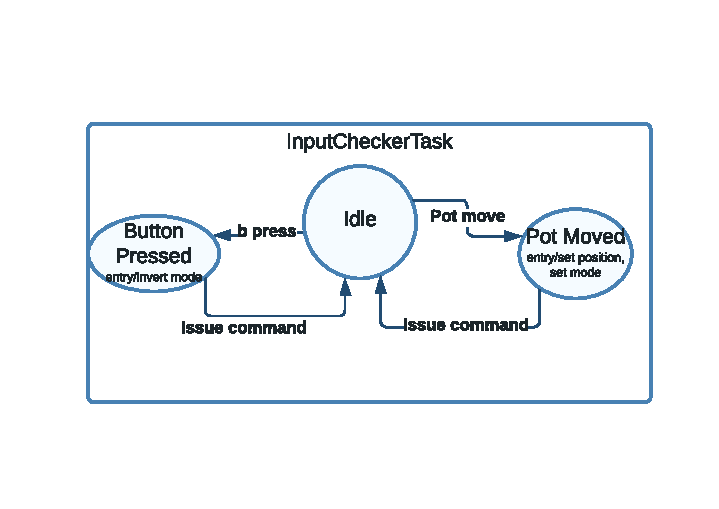
\includegraphics[width=0.8\textwidth]{InputChecker.pdf}
\end{figure}
\subsection{displayFeedback Task}
This task displaies the active status of the machine (auto/manual) and the position of the valve message on the LCD display.
